% !TEX root = ../../main.tex

\section{Physical models of adsorption}%
\label{pyg:models}

As the process of characterisation of porous materials
relies on mathematical models of how adsorption
takes place inside the pores, this section details
several such concepts.

A lot of effort was put into attempting to describe
the phenomenon of adsorption. Through a well-defined
model, the underlying mechanisms of adsorption can be
understood. Unfortunately, the plethora of isotherm
features and shapes can only be truly recreated
by molecular simulation, which requires an exact
knowledge of the adsorbent structure and its interaction
with the guest molecules. 
Nevertheless, simple models derived from a kinetic or thermodynamic
view of adsorption can be useful for obtaining simple parameters
which are representative of physical factors such as
guest-host interaction, surface area, pore size,
and total capacity.

Isotherm models which have a thermodynamical basis are derived
from the Gibbs equation (\autoref{pyg:eqn:gibbs}). This approach
describes adsorption in terms of a surface excess with respect 
to the bulk gas phase. The pressure and volume concepts of the bulk phase
are replaced by the 2-dimensional analogues of spreading pressure (\( \pi \))
and surface area.

\begin{equation}\label{pyg:eqn:gibbs}
	\Big(\frac{d\pi}{d\ln{p}}\Big) = \frac{n}{A} R_g T
\end{equation}

By substituting spreading pressure with an equation
of state for the adsorbed phase, an expression for the amount
adsorbed can be obtained as a function of bulk phase pressure.
Models which are derived from this equation include
Henry's law, the virial model and vacancy solution theory.

Adsorption can also be described a kinetic standpoint, where 
the rate of adsorption and desorption of molecules on 
available sites is mathematically modelled. Equations based
on kinetics include the Langmuir model, the BET model
the Temkin model and empirical or semi-empirical derivatives 
such as the Toth, Quadratic or the Jensen-Seaton model.

A page of figures for different models with several
values of their parameter can be seen in
\autoref{pyg:fgr:modelex}.


\begin{figure}[p]
	\centering

	\begin{subfigure}{0.3\linewidth}

		\parbox[c]{1.0\linewidth}{\caption{Henry}%
			\label{pyg:fgr:henryex}}

		\parbox[b]{1.0\linewidth}{%

			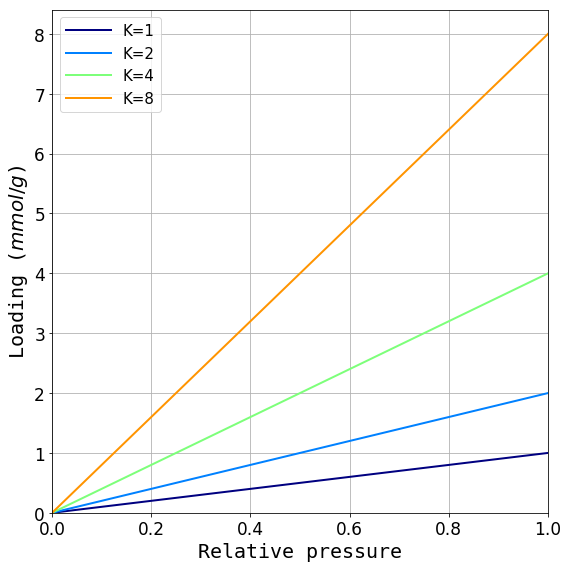
\includegraphics[width=\linewidth]{models/henry}}
	\end{subfigure}%
	\begin{subfigure}{0.3\linewidth}

		\parbox[c]{1.0\linewidth}{\caption{Langmuir}%
			\label{pyg:fgr:langmuirex}}

		\parbox[b]{1.0\linewidth}{%

			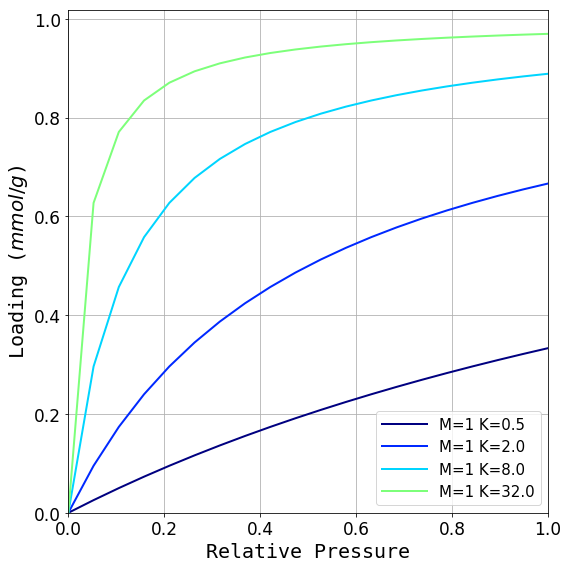
\includegraphics[width=\linewidth]{models/langmuir}}
	\end{subfigure}%
	\begin{subfigure}{0.3\linewidth}

		\parbox[c]{1.0\linewidth}{\caption{BET}%
			\label{pyg:fgr:betex}}

		\parbox[b]{1.0\linewidth}{%

			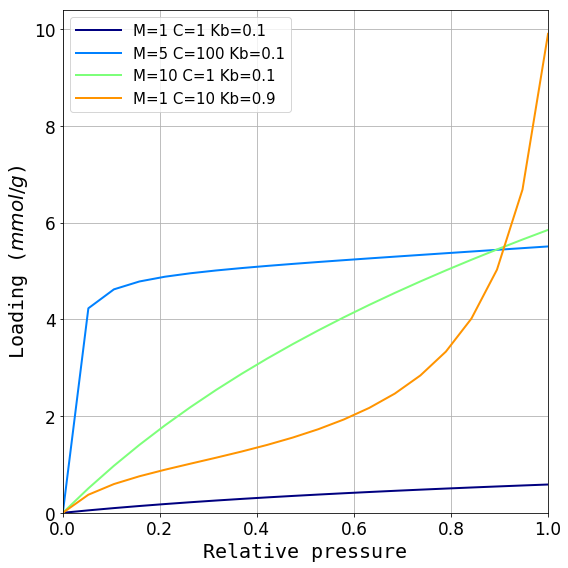
\includegraphics[width=\linewidth]{models/bet}}
	\end{subfigure}%

	\begin{subfigure}{0.3\linewidth}

		\parbox[c]{1.0\linewidth}{\caption{Toth}%
			\label{pyg:fgr:tothex}}

		\parbox[b]{1.0\linewidth}{%

			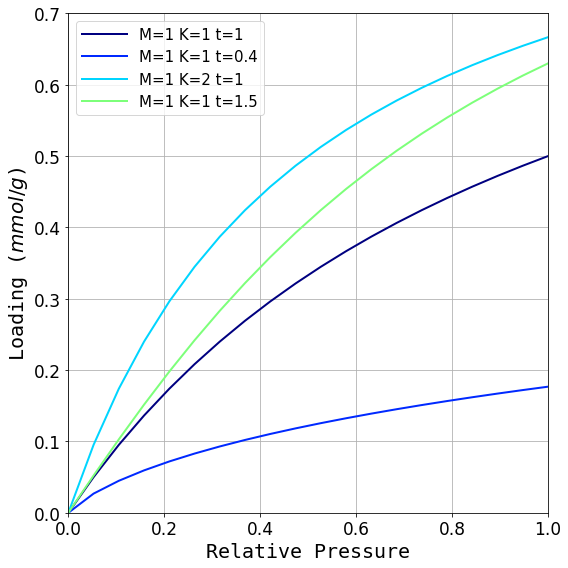
\includegraphics[width=\linewidth]{models/toth}}
	\end{subfigure}%
	\begin{subfigure}{0.3\linewidth}

		\parbox[c]{1.0\linewidth}{\caption{Quadratic}%
			\label{pyg:fgr:quadraticex}}

		\parbox[b]{1.0\linewidth}{%

			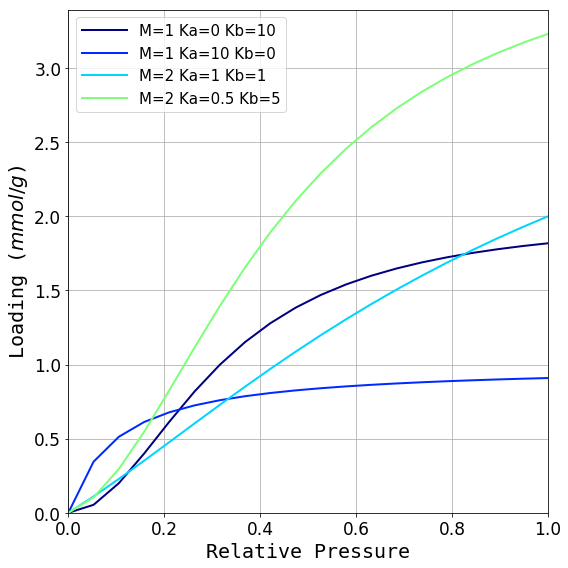
\includegraphics[width=\linewidth]{models/quadratic}}
	\end{subfigure}%
	\begin{subfigure}{0.3\linewidth}

		\parbox[c]{1.0\linewidth}{\caption{Jensen Seaton}%
			\label{pyg:fgr:jseatonex}}

		\parbox[b]{1.0\linewidth}{%

			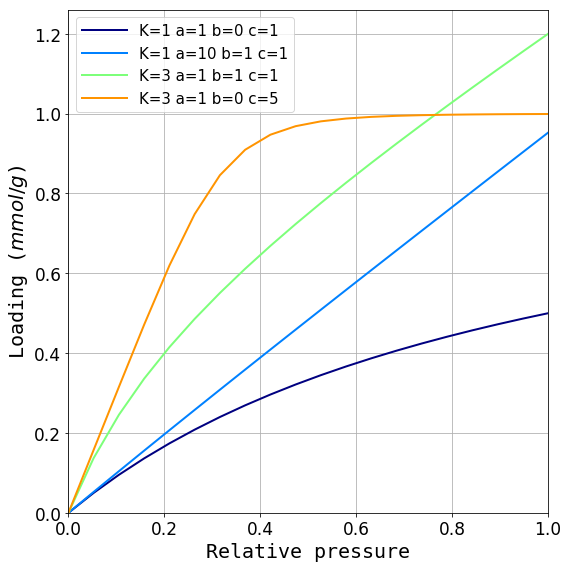
\includegraphics[width=\linewidth]{models/jseaton}}
	\end{subfigure}%
	\\
	\begin{subfigure}{0.3\linewidth}

		\parbox[c]{1.0\linewidth}{\caption{Temkin}%
			\label{pyg:fgr:temkinex}}

		\parbox[b]{1.0\linewidth}{%

			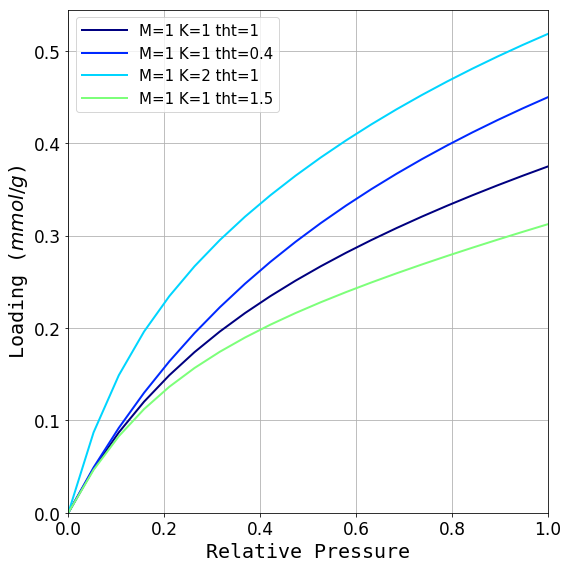
\includegraphics[width=\linewidth]{models/temkin}}
	\end{subfigure}%
	\begin{subfigure}{0.3\linewidth}

		\parbox[c]{1.0\linewidth}{\caption{Virial}%
			\label{pyg:fgr:virialex}}

		\parbox[b]{1.0\linewidth}{%

			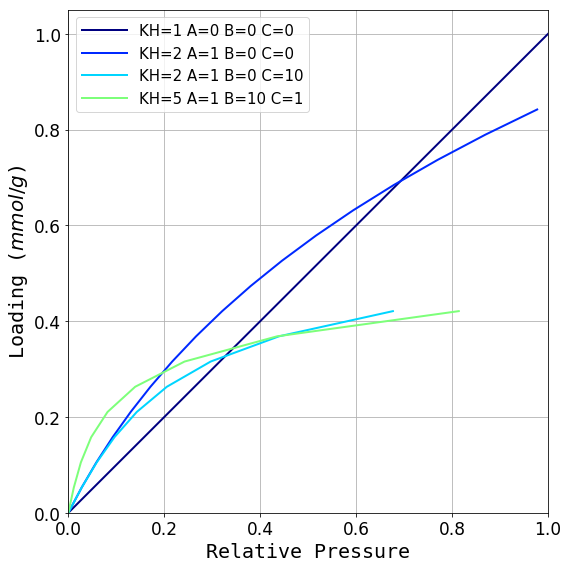
\includegraphics[width=\linewidth]{models/virial}}
	\end{subfigure}%
	\begin{subfigure}{0.3\linewidth}

		\parbox[c]{1.0\linewidth}{\caption{W-VST}%
			\label{pyg:fgr:wsvstex}}

		\parbox[b]{1.0\linewidth}{%

			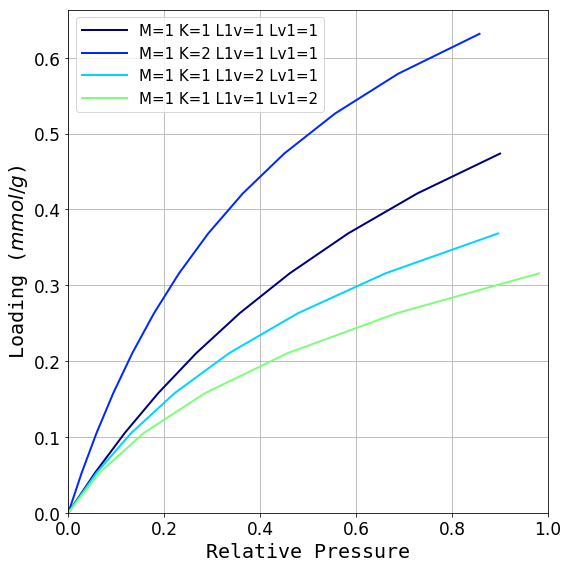
\includegraphics[width=\linewidth]{models/wvst}}
	\end{subfigure}%
	\\
	\begin{subfigure}{0.3\linewidth}

		\parbox[c]{1.0\linewidth}{\caption{FH-VST}%
			\label{pyg:fgr:fhvstex}}

		\parbox[b]{1.0\linewidth}{%

			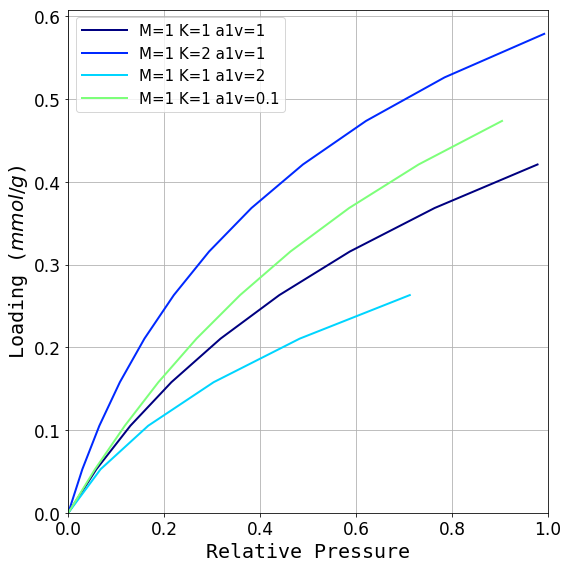
\includegraphics[width=\linewidth]{models/fhvst}}
	\end{subfigure}%

	\caption{Examples of models
	}%
	\label{pyg:fgr:modelex}
\end{figure}

\subsection{The Henry model}\label{pyg:models:henry}

The simplest method of describing adsorption on a
surface is Henry’s law. It assumes only interactions
with the adsorbate surface and is described by a
linear dependence of adsorbed amount with
increasing pressure.

\begin{equation}\label{pyg:eqn:henry}
	n_a(p) = K_H p
\end{equation}

It is derived from the Gibbs isotherm, by substituting a
a two dimensional analogue to the ideal gas law.
From a physical standpoint, Henry's law is unrealistic as adsorption sites
will saturate at higher pressures. However, the constant \(K_H\),
or Henry’s constant, can be thought of as a measure of the strength
of the interaction of the probe gas with the surface. At very
low concentrations of gas there is a
theoretical requirement for the applicability of Henry's law.
Therefore, most models reduce to \autoref{pyg:eqn:henry}
as \(\lim_{p \to 0} n(p)\).

\subsection{Langmuir and multi-site Langmuir
	model}\label{pyg:models:langmuir}

The Langmuir theory~\cite{langmuirAdsorptionGasesPlane1918},
proposed at the start of the 20th century, states that
adsorption takes place on specific sites on a surface, until
all sites are occupied.
It is derived from a kinetic model of gas adsorption and
is based on several assumptions.

\begin{itemize}

	\item All sites are equivalent and have the same chance of
	      being occupied.
	\item Each adsorbate molecule can occupy one adsorption site.
	\item There are no interactions between adsorbed molecules.
	\item The rates of adsorption and desorption are proportional
	      to the number of sites currently free and currently occupied,
	      respectively.
	\item Adsorption is complete when all sites are filled.

\end{itemize}

Using these assumptions we can define rates for both adsorption and
desorption. The adsorption rate (\autoref{pyg:eqn:langmuir_ads})
will be proportional to the number of sites available on the surface,
as well as the number of molecules in the gas, which is given by
pressure.
The desorption rate, on the other hand, will be proportional to the
number of occupied sites and the energy of adsorption
(\autoref{pyg:eqn:langmuir_des}).
It is also useful to define \(\theta = n_a/n_a^m\) as the surface
coverage,
the number of sites occupied divided by the total sites. At
equilibrium,
the rate of adsorption and the rate of
desorption are equal, therefore the two equations can be combined.
The equation can then be arranged to obtain an expression for the
loading called the Langmuir model (\autoref{pyg:eqn:langmuir}).

\begin{align}
	v_a                & = k_a p (1 - \theta) \label{pyg:eqn:langmuir_ads} \\
	v_d                & = k_d \theta \exp{\Big(-\frac{E_{ads}}{RT}\Big)}
	\label{pyg:eqn:langmuir_des}                                           \\
	v_a                & = v_d                                             \\
	k_a p (1 - \theta) & = k_d \theta \exp{\Big(-\frac{E_{ads}}{RT}\Big)}        \\
	n_a(p)             & = n_a^m \frac{Kp}{1+Kp} \label{pyg:eqn:langmuir}
\end{align}

The Langmuir constant \(K\) is the product of the individual
desorption and adsorption constants \(k_a\) and \(k_d\) and exponentially
related to the energy of adsorption \(E_{ads}\).

A common extension to the Langmuir model is to consider
the experimental isotherm to be the sum of several Langmuir-type
isotherms, each with specific maximum coverage and affinities.
The underlying assumption is that the adsorbent has several distinct
types of homogeneous adsorption sites and a Langmuir
equation is used for each. This is particularly
applicable in cases where the structure of the adsorbent
suggests that different types of sites are present,
such as in crystalline materials of variable chemistry like
zeolites and MOFs. The resulting isotherm equation becomes:

\begin{equation}\label{pyg:eqn:langmulti}
	n_a(p) = \sum_i n_{a,i}^m\frac{K_i p}{1+K_i p}
\end{equation}

In practice, only up to three adsorption sites are usually
considered.

\subsection{BET model}\label{pyg:models:bet}

Like the Langmuir mode, The BET model~\cite{brunauerAdsorptionGasesMultimolecular1938}
assumes that adsorption is kinetically driven and takes place on adsorption
sites at the material surface. However, each adsorbed molecule becomes,
in itself a secondary adsorption site, such that incremental layers
are formed. The conditions imagined by the BET model are:

\begin{itemize}
	\item The surface adsorption sites are equivalent, and therefore the
	      surface is considered heterogeneous.
	\item There are no lateral interactions between adsorbed
		  molecules.
	\item The adsorption occurs in layers, with adsorbed
	      molecules acting as sites for the next layer.
\end{itemize}

A percentage of the surface \(\theta_x\) is occupied with
x layers. For each layer at equilibrium, the adsorption and
desorption rates must be equal.
The Langmuir model is then applied for each of layer
as shown in \autoref{pyg:tab:bet-deriv}. It is assumed
that the adsorption energy of a molecule on the second
and higher layers is just the condensation energy of the
adsorbent \(E_{i>1} = E_L\). Since it follows that
all layers beside the first have the same properties,
we can also define \(g= {k_{d_2}}{k_{a_2}} = {k_{d_3}}{k_{a_3}} =
\cdots\).

\begin{table}[h]
	\centering
	\caption{Derivation of the BET method from each adsorbed layer}%
	\label{pyg:tab:bet-deriv}
	\begin{tabular}{cc}
		\toprule
		All layers                                        & Re-arranged \\
		\midrule
		\parbox{0.4\textwidth}{\begin{align*}
				k_{a_1} p \theta_0     & = k_{d_1} \theta_1
				\exp{\Big(-\frac{E_1}{RT}\Big)}             \\
				k_{a_2} p \theta_1     & = k_{d_2} \theta_2
				\exp{\Big(-\frac{E_2}{RT}\Big)}             \\
				k_{a_2} p \theta_2     & = k_{d_3} \theta_3
				\exp{\Big(-\frac{E_3}{RT}\Big)}             \\
				\vdots                                      \\
				k_{a_i} p \theta_{i-1} & = k_{d_i} \theta_i
				\exp{\Big(-\frac{E_i}{RT}\Big)}
			\end{align*}} &
		\parbox{0.4\textwidth}{ \begin{align*}
				p \theta_0     & = \frac{k_{d_1}}{k_{a_1}} \theta_1
				\exp{\Big(-\frac{E_1}{RT}\Big)}                     \\
				p \theta_1     & = g \theta_2
				\exp{\Big(-\frac{E_L}{RT}\Big)}                     \\
				p \theta_2     & = g \theta_3
				\exp{\Big(-\frac{E_L}{RT}\Big)}                     \\
				\vdots                                              \\
				p \theta_{i-1} & = g \theta_i
				\exp{\Big(-\frac{E_L}{RT}\Big)}
			\end{align*}}              \\
		\bottomrule
	\end{tabular}
\end{table}

The coverage for each layer \(\theta\) can now be
expressed in terms of \(\theta_0\).

\begin{align}
	\theta_i & = \Big[p \frac{k_{a_1}}{k_{d_1}} \exp{\Big(-\frac{E_1}{RT}\Big)}\Big] x^{i-1} \theta_0
	\intertext{where}
	x        & = \frac{p}{g} \exp{\Big(-\frac{E_L}{RT}\Big)}
\end{align}

A constant C may be defined such that:

\begin{align}
	C        & = \frac{k_{a_1}}{k_{d_1}} g \exp{\Big(\frac{E_1 - E_L}{RT}\Big)} \\
	\theta_i & = C x^i \theta_0
\end{align}

For all the layers, the equations can be summed:

\begin{align}
	\frac{n}{n_m} & = \sum_{i=1}^{\infty} i \theta^i = C
	\sum_{i=1}^{\infty} i x^i \theta_0
	%
	\intertext{and since}
	%
	\theta_0      & = 1 - \sum_{1}^{\infty} \theta_i
	\sum_{i=1}^{\infty} i x^i = \frac{x}{(1-x)^2}
\end{align}

Then we obtain the BET equation:

\begin{equation}\label{pyg:eqn:bet}
	n_a(p) = n_a^m \frac{C (p/p_0)}{(1-p/p_0)[1-(p/p_0)+ C (p/p_0)]}
\end{equation}

The BET constant \(C\) is exponentially proportional to the
difference between the surface adsorption energy and the 
intermolecular attraction and can be seen to influence the ``knee''
a BET-type isotherm has at low pressure, before statistical
monolayer formation.

\subsection{Toth model}\label{pyg:models:toth}

The Toth model is an empirical modification to the Langmuir equation
(\autoref{pyg:eqn:langmuir})
which introduces a power parameter for the denominator leading to
the following equation:

\begin{equation}\label{pyg:eqn:toth}
	n_a(p) = n_a^m \frac{K p}{{[1 + {(K p)}^t]}^{1/t}}
\end{equation}

The parameter \(t\) is a measure of the system heterogeneity.
Thanks to this additional parameter, the Toth equation can
accurately describe a large number of adsorbent/adsorbate systems
and, due to its correct behaviour in both the low and high pressure
limits, is recommended as the fitting isotherms of many
adsorbents such as hydrocarbons, carbon oxides, hydrogen sulphide
and alcohols on activated carbons and zeolites.

\subsection{Temkin model}\label{pyg:models:temkin}

The Temkin adsorption
isotherm~\cite{temkinKineticsAmmoniaSynthesis1940},
like the Langmuir model, considers
a surface with \(n_a^m\) identical adsorption sites, but takes into
account adsorbate-adsorbate interactions by assuming that the 
heat of adsorption is a linear function of  coverage. 
The formula in \autoref{pyg:eqn:temkin} is derived
using a mean-field argument and uses an asymptotic approximation
to obtain an explicit equation for the
loading~\cite{simonOptimizingNanoporousMaterials2014}.

\begin{equation}\label{pyg:eqn:temkin}
	n_a(p) = n_a^m \frac{Kp}{1+Kp} + n_a^m \theta
	{\Big(\frac{Kp}{1+Kp}\Big)}^2 \Big(\frac{Kp}{1+Kp} -1\Big)
\end{equation}

Here, \(n_a^m\) and K have the same physical meaning as in the
Langmuir model.
The additional parameter \(\theta\) describes the strength of the
adsorbate-adsorbate
interactions (\(\theta < 0\) for attractions).

\subsection{Jensen-Seaton model}\label{pyg:models:jseaton}

When modelling supercritical adsorption in micropores, a requirement was
highlighted by
Jensen and Seaton in 1996~\cite{jensenIsothermEquationAdsorption1996}
that at sufficiently high pressures the adsorption
isotherm should not reach a horizontal plateau corresponding to
saturation but that this asymptote should continue to rise due to 
the compression of the adsorbate in the pores. They developed a 
semi-empirical equation to describe this phenomenon based on a function
that interpolates between two asymptotes: the Henry’s law asymptote at
low pressure and an asymptote reflecting the compressibility of
the adsorbate at high pressure.

\begin{equation}\label{pyg:eqn:jseaton}
	n(p) = K_H p \Big{(1 + \frac{K_H p}{{[a {(1 + b
									p)}]}^c}\Big)}^{(-1/c)}
\end{equation}

Here \(K_H\) is the Henry constant, \(b\) is the compressibility of
the adsorbed phase and \(c\) an empirical constant.

The equation can be used to model both absolute and excess adsorption
as the pore volume can be incorporated into the definition of \(b\), 
although this can lead to negative adsorption slopes for the 
compressibility asymptote. This equation has been found to provide a 
better fit for experimental data from microporous solids than the 
Langmuir or Toth equation, in particular for
adsorbent/adsorbate systems with high Henry’s constants where the
amount adsorbed increases rapidly at relatively low pressures and
then slows down dramatically.

\subsection{Quadratic model}\label{pyg:models:quadratic}

The quadratic adsorption
isotherm~\cite{hillIntroductionStatisticalThermodynamics1986}
exhibits an inflection point. The loading is convex at low
pressures but changes concavity as it saturates, yielding
an S-shape. The S-shape can be explained by adsorbate-adsorbate
attractive forces: the initial convexity is due to a cooperative
effect of adsorbate-adsorbate attractions aiding in the recruitment
of additional adsorbate molecules.

\begin{equation}\label{pyg:eqn:quad}
	n(p) = n_a^m \frac{(K_a + 2 K_b p)p}{1+K_{ap} + K_{bp}^2}
\end{equation}

The parameter \(K_a\) can be interpreted as the Langmuir constant;
the strength of the adsorbate-adsorbate attractive forces is 
embedded in \(K_b\). It is often useful in systems where the 
energy of guest-guest interactions is actually higher than
the energy of adsorption, such as when adsorbing water 
on a hydrophobic surface.

\subsection{Virial model}\label{pyg:models:virial}

A virial isotherm model attempts to fit the measured data to a
factorized exponent relationship between loading and
pressure~\cite{myersThermodynamicsAdsorptionPorous2002}.

\begin{equation}\label{pyg:eqn:virial}
	p = n \exp{(K_1n^0 + K_2n^1 + K_3n^2 + K_4n^3 + \cdots + K_i
		n^{i-1})}
\end{equation}

It has been applied with success to describe the behaviour of
standard as well as supercritical isotherms. The factors are 
usually empirical, although some relationship with physical 
properties can be determined:
the first constant is related to the Henry constant at
zero loading, while the second constant is a measure of the 
interaction strength with the surface.

\begin{equation}
	K_1 = -\ln{K_{H,0}}
\end{equation}

In practice, besides the first constant, only 2--3 factors are used.

\subsection{Vacancy solution theory models}\label{pyg:models:vst}

As a part of the Vacancy Solution Theory (VST) family of models, 
it is based on concept of a “vacancy” species, denoted v, and 
assumes that the adsorbed phase is analogue to a mixture of these
vacancies and the adsorbate. \todo{rewrite}

The VST model is defined as follows:

\begin{itemize}

	\item A vacancy is an imaginary entity defined as a vacuum
	      space which acts as the solvent in both the gas and adsorbed
	      phases.
	\item The properties of the adsorbed phase are defined as
	      excess properties in relation to a dividing surface.
	\item The entire system including the adsorbent are in
	      thermal equilibrium however only the gas and adsorbed phases are in
	      thermodynamic equilibrium.
	\item The equilibrium of the system is maintained by the
	      spreading pressure
	      which arises from a potential field at the surface

\end{itemize}

It is possible to derive expressions for the vacancy chemical
potential in both the adsorbed phase and the gas phase, which when
equated give the following equation of state for the adsorbed phase:

\begin{equation}
	\pi = - \frac{R_g T}{\sigma_v} \ln{y_v x_v}
\end{equation}

where \(y_v\) is the activity coefficient and  \(x_v\) is the mole
fraction of the vacancy in the adsorbed phase.
This can then be introduced into the Gibbs equation to give a general
isotherm equation for the Vacancy Solution Theory where \(K_H\) 
is the Henry’s constant and
\(f(\theta)\) is a function that describes the non-ideality of the
system based on activity coefficients:

\begin{equation}
	p = \frac{n_{ads}}{K_H} \frac{\theta}{1-\theta} f(\theta)
\end{equation}

The general VST equation requires an expression for the activity
coefficients. The Wilson~\cite{suwanayuenGasAdsorptionIsotherm1980} 
equation can be used, which expresses the activity coefficient in terms
of the mole fractions of the two species (adsorbate and vacancy) and
two constants \(\Lambda_{1v}\) and \(\Lambda_{1v}\). The equation
then becomes:

\begin{equation}\label{pyg:eqn:wvst}
	p = \bigg( \frac{n_{ads}}{K_H} \frac{\theta}{1-\theta} \bigg)
	\bigg( \Lambda_{1v}
	\frac{1-(1-\Lambda_{v1})\theta}{\Lambda_{1v}+(1-\Lambda_{1v})\theta}
	\bigg)
	\exp{\bigg(
		-\frac{\Lambda_{v1}(1-\Lambda_{v1})\theta}{1-(1-\Lambda_{v1})\theta}
		-\frac{(1 - \Lambda_{1v})\theta}{\Lambda_{1v} +
			(1-\Lambda_{1v}\theta)} \bigg)}
\end{equation}

Cochran~\cite{cochranVacancySolutionTheory1985} developed a simpler, 
three parameter equation based on the Flory–Huggins equation for the 
activity coefficient. The equation for then becomes:

\begin{equation}\label{pyg:eqn:fhvst}
	p = \bigg( \frac{n_{ads}}{K_H} \frac{\theta}{1-\theta} \bigg)
	\exp{\frac{\alpha^2_{1v}\theta}{1+\alpha_{1v}\theta}}
	\quad \text{where} \quad
	\alpha_{1v} = \frac{\alpha_{1}}{\alpha_{v}} - 1
\end{equation}

Here \(\alpha_{1}\) and \(\alpha_{v}\) are the molar areas of the
adsorbate and the vacancy respectively.
